\section{Diagram of the combined model}
%\begin{figure}[ht]
%    \centering
%    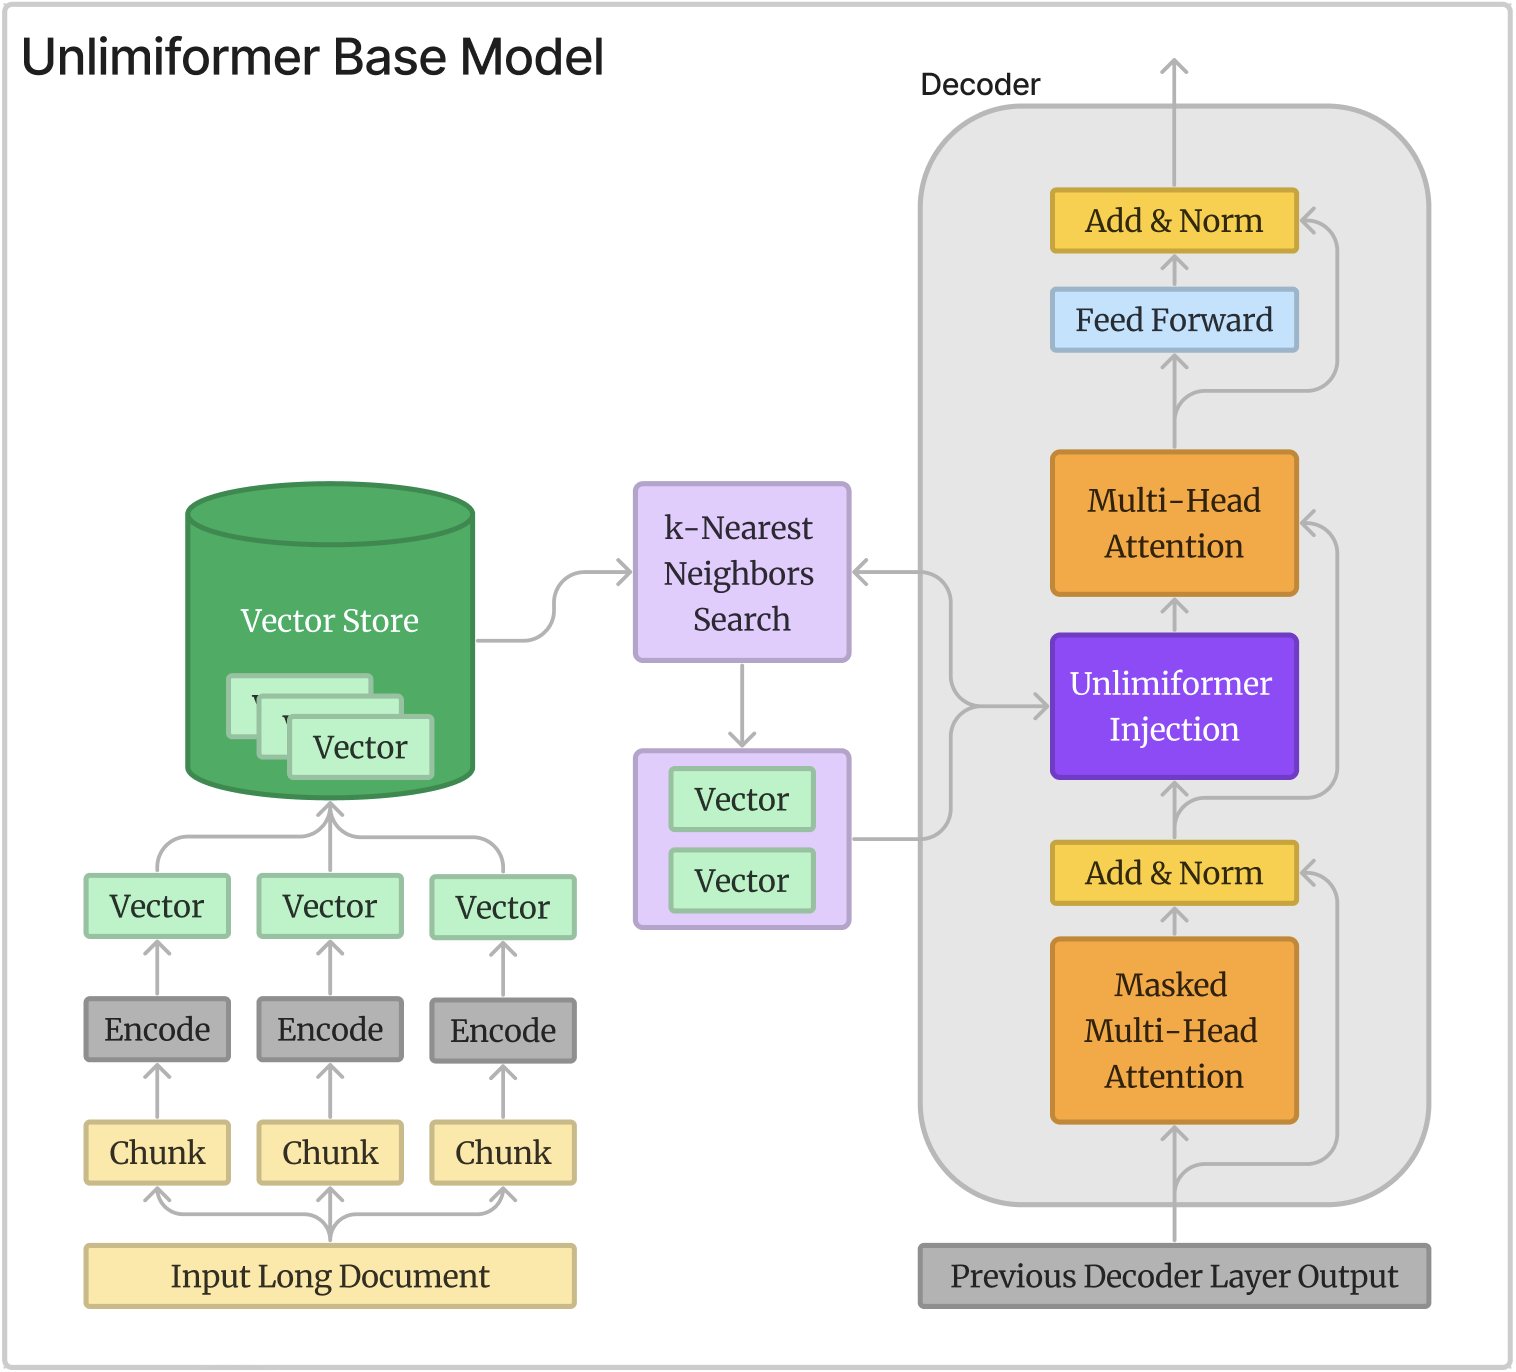
\includegraphics[scale=.27]{images/baselinemodel_2.png}
%    \caption{The baseline \texttt{unlimiformer} model}
%    \label{fig:baseline}
%\end{figure}
\begin{figure}[ht]
  \centering 
  \vskip.5cm
  \begin{tikzpicture}[node distance=1.9cm]

%-----------chunks
  \node (chunk1) [startstop] {\{{\bf a , b}\} , c , d};
  \node (chunk2) [startstop, right of=chunk1, xshift=1cm] {b , \{{\bf c , d}\} , e};
  \node (chunk3) [startstop, right of=chunk2, xshift=1cm] 
    {c , d , \{{\bf e , f}\}};
%-----------the long document
\node[draw, rectangle, minimum width=4cm, minimum height=1cm,
  below of=chunk2]
  (longdoc) [startstop]{LongDoc = \{a , b , c , d , e , f\}};
%-----------the encoder
\node (encoder)[decision, above of=chunk2, xshift=0cm] {Standard Encoder};

%-----------the attention mechanism
\node (attn) [standardFn, right of=encoder, xshift=3cm] {Attention};

%-----------unlimiformer-----------
%-----------the datastore
\node[draw, rectangle, fill=red!30, minimum width=4cm, minimum height=1cm,
  above of=encoder, xshift=0cm, rounded corners]
  (datastore) {Datastore of LongDoc in $\mathcal H_\text{enc}$};
%-----------selecting the k nearest
\node (nearest) [unlimiFn, above of=attn] {$4$ ``nearest''};

%-----------combined model
\node[draw, rectangle, fill=green!30, minimum width=4cm, minimum height=1cm,
  above of=datastore, rounded corners]
  (kg) {Encoded representation of KG
%    $2^{\mathcal H_\text{enc}} \times 2^{\mathcal H_\text{enc}}$
  };
%-----------the alternative search
\node (search) [combFn, above of=nearest] {graph search};
%

%-----------decoder
\node (decoder2) [decision, right of=attn, xshift=2cm, yshift=0cm]
  {Decoder};
%-----------decoder
\node (decoder1) [decision, below of=decoder2]
  {Layers};
%-----------decoder
\node (decoder3) [decision, above of=decoder2]
  {Standard};

%-----------partial summary
\node (parsum) [startstop, below of=decoder1] {Partial Summary};
%-----------final summary
\node (sum) [startstop, above of=decoder3] {Summary};

\draw [arrow] (longdoc) -- (chunk1);
\draw [arrow] (longdoc) -- (chunk2);
\draw [arrow] (longdoc) -- (chunk3);
\draw [arrow] (chunk1) -- (encoder);
\draw [arrow] (chunk2) -- (encoder);
\draw [arrow] (chunk3) -- (encoder);
\draw [arrow] (encoder) -- (datastore);
\draw [arrow] (datastore) -- (kg);
\draw [arrow] (datastore) -- (nearest);
\draw [arrow] (kg) -- (search);
\draw [arrow] (search) -- (nearest);
\draw [arrow] (nearest) -- (attn);
\draw [arrow] (decoder1) -- (attn);
\draw [arrow] (decoder2) -- (attn);
\draw [arrow] (decoder3) -- (attn);
\draw [arrow] (attn) -- (decoder3);
\draw [arrow] (attn) -- (decoder1);
\draw [arrow] (attn) -- (decoder2);
\draw [arrow] (attn) -- (decoder3);
\draw [arrow] (encoder) -- (attn);
\draw [arrow] (parsum) -- (decoder1);
\draw [arrow] (decoder1) -- (decoder2);
\draw [arrow] (decoder2) -- (decoder3);
\draw [arrow] (decoder3) -- (sum);

\end{tikzpicture}
\caption{\footnotesize A stylised transformer with length-$4$ context window
  (in blue).  The standard approach to handling long documents is to process
  consecutive overlapping chunks of tokens sequentially. In red,
  \texttt{unlimiformer} augments this process by creating a complete datastore
  and selecting which tokens are fed into the attention mechanism. We augment this
process further using a Knowledge Graph to aid selection.} \label{fig-latex}
\end{figure}

%\begin{figure}[ht]
%  \centering 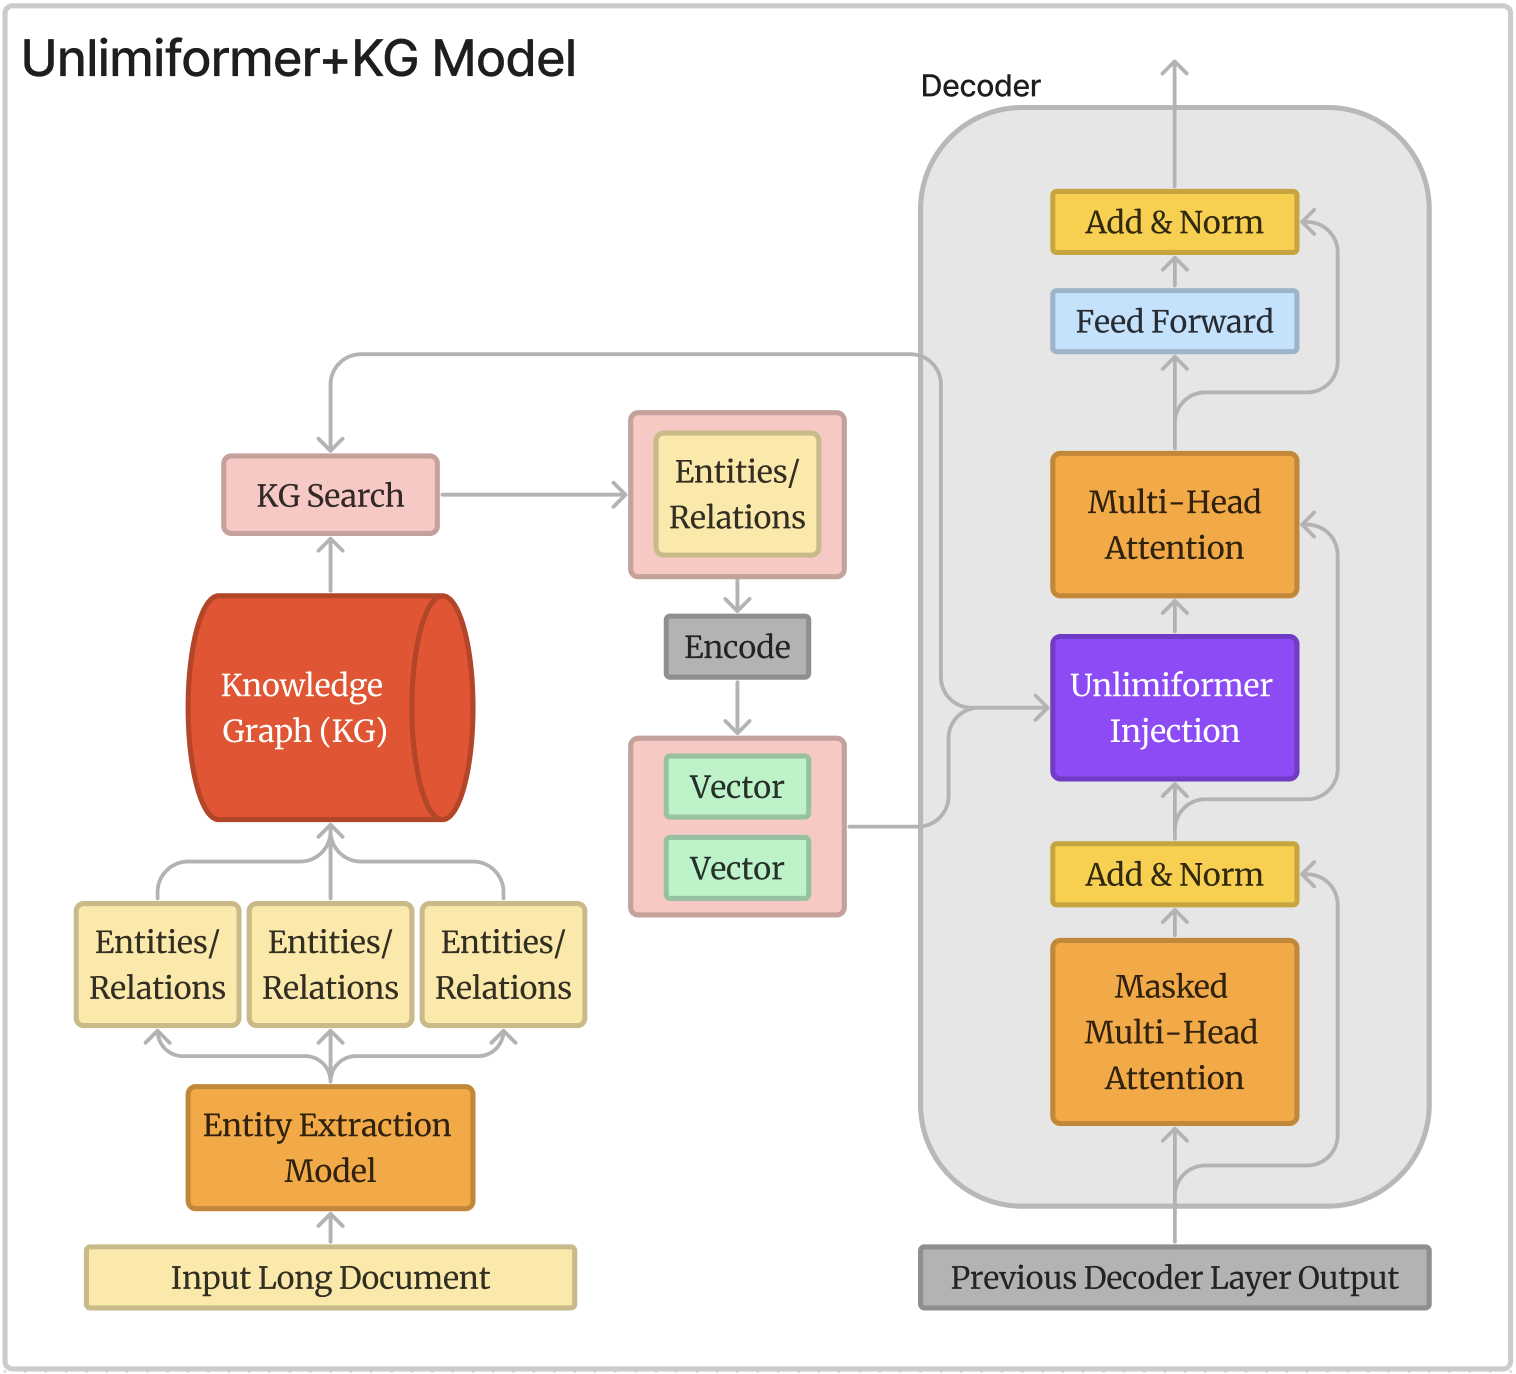
\includegraphics[scale=0.27]{images/combinedmodel_2.png}
%  \caption{Building the KG via entity extraction and a slightly different
%  architecture}
%  \label{fig-extraction}
%\end{figure}

%
%\begin{tikzpicture}[node distance=1cm, auto, 
%    box/.style={draw, rectangle, minimum width=1cm, minimum height=0.8cm, align=center},
%    every path/.style={-latex, thick}]
%
%% Nodes
%\node[draw, rectangle, fill=gray!30, minimum width=4cm, minimum height=1cm] (input) {Index of one long input};
%\node[draw, rectangle, below=2cm of input] (encoder) {Encoder};
%\node[draw, rectangle, fill=green!30, right=2.5cm of encoder] (knn) {kNN Search};
%\node[draw, rectangle, fill=green!30, above right=0.5cm and 1cm of knn] (query) {query};
%\node[box, below=1cm of encoder] (a1) {a};
%\node[box, right=0.1cm of a1] (b1) {b};
%\node[box, right=0.1cm of b1] (c1) {c};
%\node[box, right=0.1cm of c1] (d1) {d};
%\node[box, right=0.1cm of d1] (e1) {e};
%\node[box, right=0.1cm of e1] (f1) {f};
%\node[box, below=1cm of a1] (a2) {a};
%\node[box, right=0.1cm of a2] (b2) {b};
%\node[box, right=0.1cm of b2] (c2) {c};
%\node[box, right=0.1cm of c2] (d2) {d};
%\node[box, right=0.1cm of d2] (e2) {e};
%\node[box, right=0.1cm of e2] (f2) {f};
%
%% Connectors
%\draw[thick] (input.south) -- (encoder.north);
%\draw[thick] (encoder.east) -- (knn.west);
%\draw[thick] (knn.north) |- (query.east);
%\draw[thick] (query.west) -| (c1.north);
%\draw[dashed, thick] (query.south) -| (c2.north);
%
%\end{tikzpicture}
%\begin{tikzpicture}[node distance=1cm, auto]
%
%% Nodes
%\node[draw, rectangle, fill=gray!30, minimum width=4cm, minimum height=1cm] (input) {Index of one long input};
%\node[draw, rectangle, below=of input, minimum width=2cm, minimum height=1cm] (encoder) {Encoder};
%\node[draw, rectangle, right=2cm of encoder, fill=green!30, minimum width=2cm, minimum height=1cm] (knn) {kNN Search};
%\node[draw, rectangle, right=2cm of knn, minimum width=2cm, minimum height=1cm] (decoder) {Decoder Layer};
%\node[draw, rectangle, below=of decoder, fill=blue!30, minimum width=2cm, minimum height=1cm] (cross) {Cross attention};
%\node[draw, rectangle, below=2cm of knn, fill=green!30, minimum width=1cm, minimum height=0.8cm] (query) {query};
%
%% etc... you would continue to define the rest of the nodes similarly
%
%% Connectors
%\draw[-{Triangle[width=3mm,length=3mm]}, thick] (input) -- (encoder);
%\draw[-{Triangle[width=3mm,length=3mm]}, thick] (encoder) -- (knn);
%% etc... you would continue to define the rest of the arrows similarly
%
%\end{tikzpicture}
%
%\begin{tikzpicture}[node distance=1cm, auto,
%    box/.style={draw, rectangle, minimum width=1cm, minimum height=0.8cm},
%    bigbox/.style={draw, rectangle, minimum width=3cm, minimum height=1.5cm},
%    every path/.style={-latex, thick}]
%
%% Nodes
%\node[draw, rectangle, fill=gray!30, minimum width=4cm, minimum height=1cm]
%  (input) {Index of one long input};
%\node[bigbox, below=1.5cm of input] (encoder) {Encoder};
%\node[bigbox, right=2cm of encoder, fill=green!30] (knn) {kNN Search};
%\node[bigbox, right=2cm of knn] (decoder) {Decoder Layer};
%\node[draw, rectangle, below=1.5cm of decoder, fill=blue!30, minimum width=2cm, minimum height=1cm] (cross) {Cross attention};
%\node[box, below=0.5cm of knn, fill=green!30] (query) {query};
%\node[box, left=0.5cm of query] (state) {Retrieved hidden states};
%\node[box, below=3cm of encoder, yshift=0.5cm] (a1) {a};
%\node[box, right=0.1cm of a1] (b1) {b};
%\node[box, right=0.1cm of b1] (c1) {c};
%\node[box, right=0.1cm of c1] (d1) {d};
%\node[box, right=0.1cm of d1] (e1) {e};
%\node[box, right=0.1cm of e1] (f1) {f};
%
%% Connectors
%\draw[thick]  (encoder.north) -- ++(0,0.5cm) -| (input.south);
%\draw[thick] (encoder) -- (knn);
%\draw[thick] (knn) -- (decoder);
%\draw[thick] (decoder.south) -- ++(0,-0.5cm) -| (cross.north);
%\draw[thick] (knn.south) -- (query);
%\draw[thick, dashed] (query) -- (state);
%\draw[thick, dashed] (query) -- (c1);
%
%% Add more connectors and nodes as requigray
%
%\end{tikzpicture}
